\documentclass[10pt]{beamer}

\usepackage[utf8]{inputenc}
\usepackage[spanish, es-tabla]{babel}

\usetheme{metropolis}
\usepackage{appendixnumberbeamer}

\usepackage{booktabs}
\usepackage[scale=2]{ccicons}

\usepackage{pgfplots}
\usepgfplotslibrary{dateplot}

\usepackage{caption}
\usepackage{subcaption}

\usepackage{graphicx}

\usepackage{amsmath}
\usepackage{amsfonts}
\usepackage{amssymb}
\usepackage{amsthm}
\usepackage{esvect}

\usepackage{multimedia}

\usepackage{xspace}
\newcommand{\themename}{\textbf{\textsc{metropolis}}\xspace}

\title{Detección de anomalías basada en técnicas de ensembles}
\author{Ignacio Aguilera Martos}
\date{\today}
\institute{Trabajo Fin de Grado \\ \href{https://github.com/nacheteam/Ensemble-Outlier-Analysis}{Código disponible en GitHub}}

\begin{document}

\maketitle

\begin{frame}[fragile]{Contenidos}
  \setbeamertemplate{section in toc}[sections numbered]
  \tableofcontents[hideallsubsections]
\end{frame}

\section{Concepto de anomalía basado en distancias}

\begin{frame}[fragile]{Tukey's Fences}
\vspace{10px}
\pause
\metroset{block=fill}

Pensado para el caso uno-dimensional.

\pause

\begin{block}{Tukey's Fences}
	Valores fuera del rango $[Q_1 - k(Q_3 - Q_1), Q_3 + k(Q_3 - Q_1)]$ con $k=1.5$
\end{block}

\pause

La propuesta de $k=1.5$ es arbitraria.

\end{frame}

\begin{frame}[fragile]{Tukey's Fences}
\vspace{10px}
\metroset{block=fill}
\centering
\movie[height = 0.8\textheight, width=0.8\textwidth, poster, showcontrols]{}{Imagenes/outlier-1d.mp4}

\end{frame}

\begin{frame}[fragile]{Tukey's Fences}
\vspace{10px}
\metroset{block=fill}

\begin{figure}
	\centering
	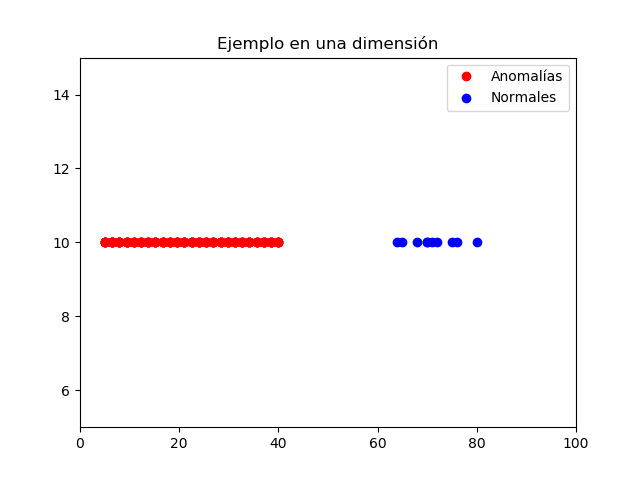
\includegraphics[scale=0.6]{Imagenes/outlier-1d.png}
\end{figure}

\end{frame}

\begin{frame}[fragile]{Extensión al caso de mayor dimensionalidad}
\vspace{10px}
\pause
\metroset{block=fill}

\begin{block}{Criterio}
	Aplicar el criterio de Tukey a cada una de las características.
	\pause
	\textbf{\underline{Trivial}}.
\end{block}

\pause

\begin{block}{Criterio de clusters}
	\begin{enumerate}
		\item Agrupamos los datos por clusters.
		\pause
		\item Encontramos el cluster más cercano para cada instancia.
		\pause
		\item Si la distancia del objeto al centroide del cluster es mayor que $1.5$ veces la mayor
		distancia intercluster entonces es una anomalía.
	\end{enumerate}
\end{block}

\end{frame}

\begin{frame}[fragile]{Ejemplo 1}
\vspace{10px}
\metroset{block=fill}
\centering
\movie[height = 0.8\textheight, width=0.8\textwidth, poster, showcontrols]{}{Imagenes/outlier-2d-case1.mp4}

\end{frame}

\begin{frame}[fragile]{Ejemplo 1}
\vspace{10px}
\metroset{block=fill}

\begin{figure}
	\centering
	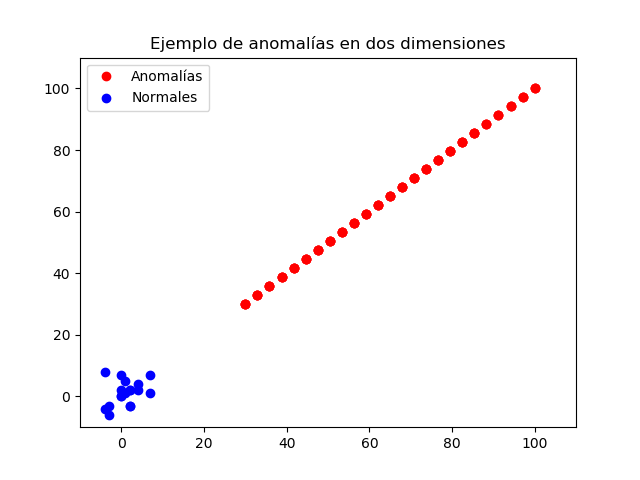
\includegraphics[scale=0.6]{Imagenes/outlier-2d-case1.png}
\end{figure}

\end{frame}

\begin{frame}[fragile]{Ejemplo 2}
\vspace{10px}
\metroset{block=fill}
\centering
\movie[height = 0.8\textheight, width=0.8\textwidth, poster, showcontrols]{}{Imagenes/outlier-2d-case2.mp4}

\end{frame}

\begin{frame}[fragile]{Ejemplo 2}
\vspace{10px}
\metroset{block=fill}

\begin{figure}
\centering
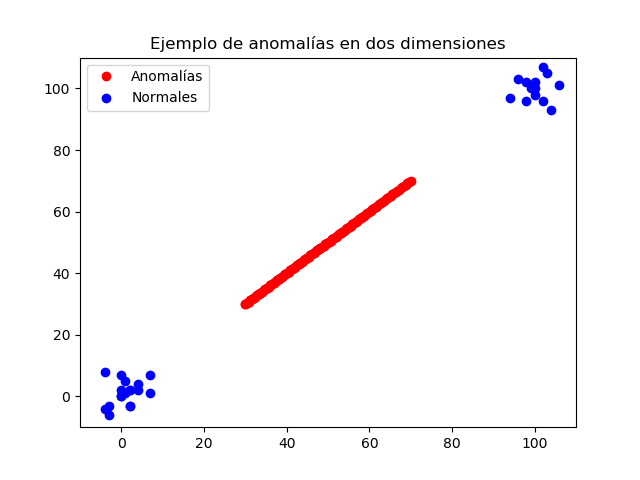
\includegraphics[scale=0.6]{Imagenes/outlier-2d-case2.png}
\end{figure}

\end{frame}

\begin{frame}[standout]
	\LARGE{¿Preguntas?}
	\vspace{10px}
\end{frame}


\end{document}
